\documentclass{article}
\usepackage[backend=bibtex]{biblatex}
\usepackage[utf8]{inputenc}
\usepackage[english]{babel}
\usepackage{caption}
\usepackage[skip=0.5ex]{subcaption}
\usepackage[left=3cm,right=3cm,top=2cm,bottom=2cm]{geometry}

\usepackage{color}
\usepackage{xcolor}
\usepackage{listings}
\definecolor{linkcolor}{rgb}{0, 0.05, 0.3}


\usepackage{hyperref}
\hypersetup{
    colorlinks=true,
    linkcolor=linkcolor,
    filecolor=magenta,      
    urlcolor=cyan,
    pdftitle={Machine Learning Exam Preparation},
    pdfpagemode=FullScreen,
    }
\usepackage{parskip} % do not indent first lines
\usepackage{bookmark}
\usepackage{booktabs}
\usepackage{textcomp}
\usepackage{array}
\usepackage{graphicx}
\usepackage{amsmath}
\usepackage{wrapfig} % wrap text around images/figures

\newcommand{\quotes}[1]{''#1''}

\graphicspath{ {./images/} }

\begin{document}
\title{Exam Preparation\\Machine Learning S. 5 Bachelor WS21/22}
\author{Jonas Weßner}
\maketitle
\tableofcontents
\newpage				% Neue Seite nach TOC

\section{Metrics for evaluating predictions}

The following metrics can be used to analyze the quality of a \textit{classification model}.

\subsection{Confusion Matrix}

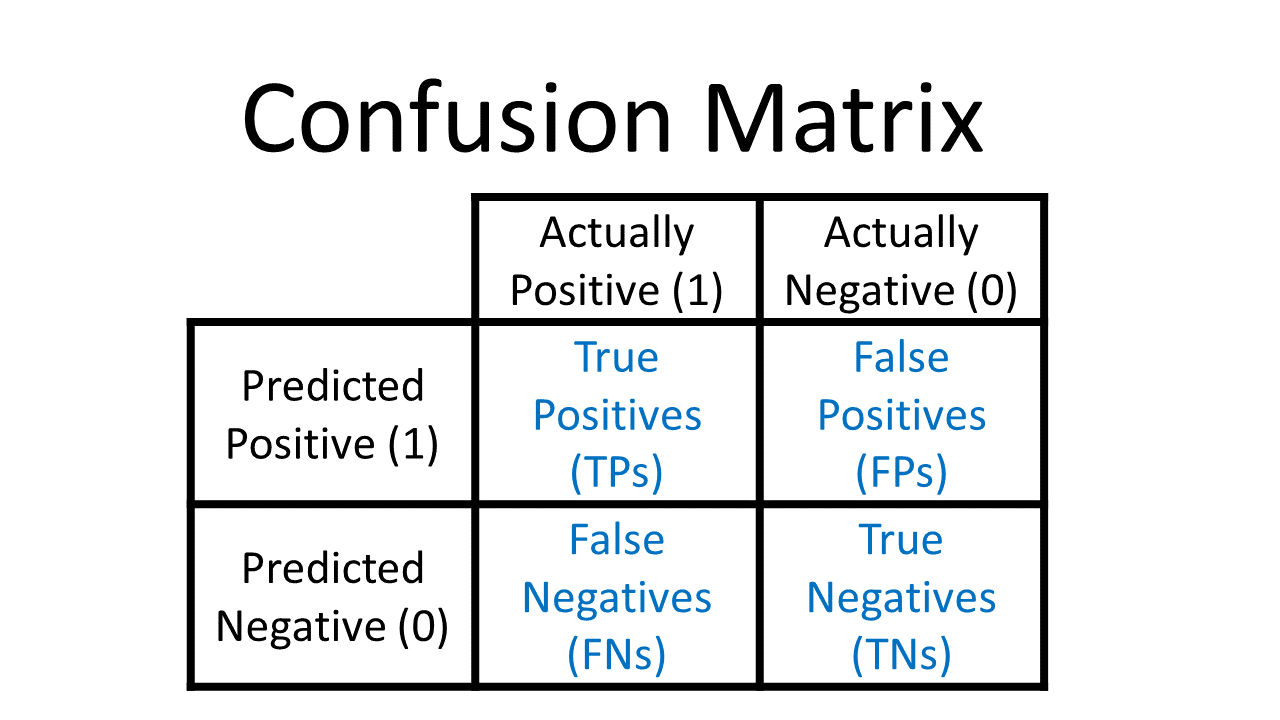
\includegraphics[width=400px]{confusion-matrix.png}

\subsection{Accuracy}

Accuracy answers the question \quotes{\textit{What is the probability that a prediciton is correct?}}.

$$
    Acc = \frac{TP + TN}{TP + TN + FP + FN}
$$

It is only good, if the real distribution of positive and negatives in the data is close to symmetric.

\subsection{Precision}

Precision answers the question \quotes{\textit{If we classify something as positive, how probable is it that it is actually positive?}}.

$$
    Precision = \frac{TP}{TP + FP}
$$

\subsection{Recall}

Recall a.k.a. sensitivity answers the question \quotes{\textit{If a sample is positive, what is the probability we also label it as positive?}}.

$$
    Recall = \frac{TP}{TP + FN}
$$

\subsection{F1 Score}

The F1-score divides the true positives by the sum of the true positives and the mean of the false positives and false negatives. This a high F1-score requires the model to make not few false predictions in either direction. Therefore F1-score is better than accuracy if the real distribution of positive and negative values in the dataset is uneven.

$$
    F1 = 2 \cdot \frac{Precision \cdot Recall}{Precision + Recall} = \frac{TP}{TP + \frac{1}{2} \cdot (FP + FN)}
$$


\section{One-hot encoding}

Many machine learning algorithms cannot have a categories as ouput values. Therefore if our goal is a categorization of samples we need to make a transformation of labels to numerical values.

\subsubsection*{Step 1: Integer Transformation}
First we must convert all different variants of the category into distinct integer values, e.g.:\\

\begin{tabular}{l l l}
    Dog         & $\rightarrow$ & 1 \\
    Cat         & $\rightarrow$ & 2 \\
    OtherAnimal & $\rightarrow$ & 3 \\
\end{tabular}

We can now train a machine learning model on that data and it will return one output value. To convert the models output back into classes we could pick the class where the ouput is the closest to the corresponding integer value.

\subsubsection*{One-Hot Encoding}

The problem with integer encoding is that we allow the model to that there is a defined order for the classes. E.g. in the above shown class mapping an ML model could assume that all other animals (3) are closer to cats (2) than to dogs (1). However, as this is not the case at all, using integer encoding might lead to poor predictions.\\
Instead we can use one-hot encoding resolving that issue. For each output class we create an output neuron / node with the value range of $[0, 1]$. The models predictions are converted back to the classes by taking the maximum of all values of the individual classes. The produces output for the individual classes can be seen as a probability that the sample is of instance of the corresponding class.

\begin{tabular}{l l l l l l}
    Dog         & $\rightarrow$ & $[0, 1]$ & $\longrightarrow$ &       \\
    Cat         & $\rightarrow$ & $[0, 1]$ & $\longrightarrow$ & $max$ \\
    OtherAnimal & $\rightarrow$ & $[0, 1]$ & $\longrightarrow$ &       \\
\end{tabular}

\section{Overfitting and Underfitting}

In supervised machine learning we usually have a function that determines a specific target parameter (e.g. if a passenger on the titanic survives). However, the function may not be accurate for all samples since the data may include errors (e.g. measurement errors). As we do not know the real underlying function we try to approximate it with supervised machine learning.\\
If a model is underfitted, it does not take all parameters of the real underlying function into account and therefore is not accurate.\\
If a model is overfitted, it takes parameters into account that do not apply to the underlying function but where given in the training samples. Overfitting leads to bad results on unseen data as parameters have been learned that are no general indicators for an event and can not be used on other data than the training samples. Overfitting may also occur if the paramters are tuned in a too detailed way that is only applicable to errors or inaccuracy of measurements in the training data.

\subsection{How can it be detected?}

To detect underfitting and overfitting we can validate the model after each training epoch by letting it make predictions on unseen data and calculating a chosen metric (in the figure we calculate a loss) over that data. Now we can make the following interpretations of the graph:

\begin{enumerate}
    \item As long as the loss is decreasing the model is still underfitted and shall be trained for more epochs.
    \item If the los is increasing the model is becoming more and more overfitted and training can be stopped.
    \item If the loss remains unchanged the model has reached the global or a local optimum.
\end{enumerate}

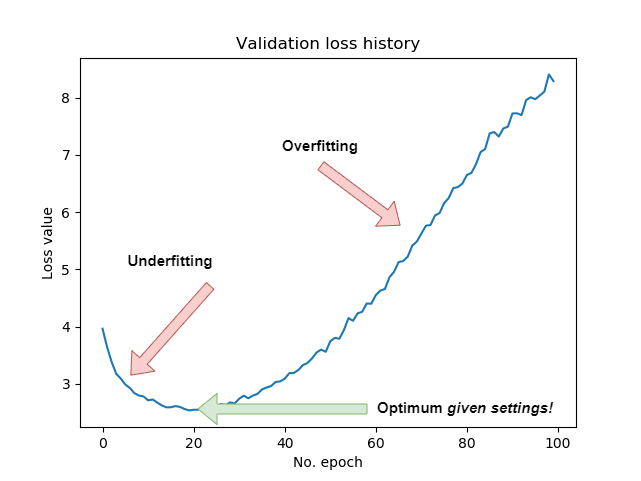
\includegraphics[width=400px]{underfitting-overfitting.png}

\subsection{Possible solutions}

\begin{enumerate}
    \item \textbf{Stop early:}\\
          Stop training to avoid overfitting if your score on the validation set does not increase anymore.
    \item \textbf{k-fold-cross-validation:}\\
          Split dataset into k groups and train k-times on k-1 groups while using the remaining group as validation data. This way after each epoch we train on data that has not been seen in that epoch while training more than one epoch.
    \item \textbf{Increase dataset size:}\\
          This has positive influence on underfitting and overfitting.
    \item \textbf{Data augmentation:}\\
          Create more data by applying some tranformations to the samples. E.g. flip and crop images. This helps preventing that the model learns too much details about individual samples.
    \item \textbf{Reduce Complexity:}\\
          Use pooling layers and less neurons to decrease overfitting.
    \item \textbf{Regularizaiton:}\\
          Penalizing big numbers of coefficients.
    \item \textbf{Use Ensembling:}\\
          Combine predictions of multiple ML-models.
\end{enumerate}

\section{PCA - principal component analysis}

\subsection{Reasons for using PCA}

If we have data with $n$ variables/features we can use principal component analysis to reduce the amount of features to $k$ with $k < n$ features while keeping the most important features of the data and eliminating the less important features. Reduction of features is useful to plot the data (because plots with more than 3 features are non-trivial) and also for machine-learning models to increase computation speed.

\subsection{Algorithm}
\begin{enumerate}
    \item Calculate mean for each variable. Doing that we also get the center of the data as $(mean(x_{1}), mean(x_{2}), ... mean(x_{n}))$.
    \item Now we want to shift the data so that its center is at the center of the coordinate system. We can subtract each individual mean from the corresponding variable to do that.
    \item We now compute the principle component 1 PC1. We are searching for a vector (straight line) that fits the data in the $x_{1}$ axis best. That means we search for a line where the squared distances of the data points to this line are minimal. It is important that this is equivalent to finding a line where the data is spread out the most if we project it onto the line.
    \item For each other variable $v_{2}$ to $v_{n}$ we draw a line that is orthogonal to all preceding lines and rotate it until it represents the data best for the given variable in the same way as with the first line. These lines are $PC_{2}$ to $PC_{n}$.
    \item As said, the data points of the features are spread out as much as possible along the PCs now. This means that the variance and therefore also the amount of information is maximized for the specific variable if we project the data onto that PC. Now we can take the $k$ PCs with the greatest variance (also called eigenvalues here) and use them to represent our data.
\end{enumerate}

\section{Python Basics}

\subsection{Slicing}

\begin{lstlisting}
    a[start:stop]       # items start through stop-1
    a[start:]           # items start through the rest of the array
    a[:stop]            # items from the beginning through stop-1
    a[:]                # a copy of the whole array
    a[start:stop:step]  # start through not past stop, by step
\end{lstlisting}

\subsection{Data Extraction with Pandas}

\begin{lstlisting}
    df.head(5)                          # show first 5 lines
    df.tail(3)                          # show last 3 lines
    df.columns              
    df.describe()                       # statistic summary of data
    df["Survived"]                      # get survived column as pandas.Series
    df[0:3]                             # get the first 3 rows with all columns
    df.loc["2013-01-03"]                # Select a row by the value of the index column
    df.loc["2013-01-03", "name"]        # Select the value of the `name` column of that row
    df.iloc[5]                          # Select the 5th row by its index
    df[df["income"] > 1000]             # selecting rows via a boolean array
    df.dropna(how="any")                # drop all rows that contain null values
    df.mean()                           # calculates mean of each column and returns a Series
    df1.fillna(value=5)                 # replace all NaN values with 5
    df.apply(lambda x: x.max() - 10)    # apply a function to each data point
\end{lstlisting}


\section{Regularization}

\label{sec:regularization}

\subsection{What is regularization}
Regularization is the method of penalizing complex model e.g. models with a lot of parameters. It is used to avoid overfitting.\\

A common loss function for evaluating a model is the residual sum of squares ($RSS$).

$$
    RSS = \sum_{i=1}^{n} (y_{i} - y'_{i})^{2}
$$

When evaluating the model the loss function shall be minimized.\\
But we can also use other loss functions that include regularization terms as will be shown in the following.

\subsection{Ridge}

Ridge adds the sum of the squares of coefficients $w$ to the RSS which makes the loss function prefer smaller coefficients. However coefficients will never be zeroed out using Ridge.

$$
    Ridge = RSS + \lambda \sum_{i=0}^{n} w_{i}^{2}
$$

\subsection{Lasso}

Lasso adds the sum of the absolutes of coefficients $w$ to the RSS which makes the loss function prefer smaller coefficients and possibly drive some coefficients to zero i.e. eliminating them.

$$
    Ridge = RSS + \lambda \sum_{i=0}^{n} |w_{i}|
$$


\subsection{Dropout}

As opposed to Ridge and Lasso, which are used mainly used with linear models, dropout is a regularization method used for neural networks. Using dropout means that the output values of some randomly chosen nodes of a layer (which may not be the output-layer) are ignored. This way the net is meant to be morel robust to noise in the training data, because it the dropped out nodes will be different in every epoch and therefore the training experience will also slightly differ.

\section{Machine Learning Tasks}

\subsection{Classification}

Classification is a \textit{supervised} machine learning task for predicting a target variable wich may have a finite number of possible values.

\subsection{Regression}

Regression is a \textit{supervised} machine learning task for predicting a continuous target variable like the price of a house or the height of a human.

\subsection{Clustering}

Clustering is an \textit{unsupervised} machine learning task for grouping data points to multiple clusters. The data points in one cluster shall be as similar as possible to each other while being as dissimilar as possible to data points in other clusters.

\section{MLP - Multi Layer Perceptron}
\label{sec:mlp}

\begin{figure}[h]
    \centering
    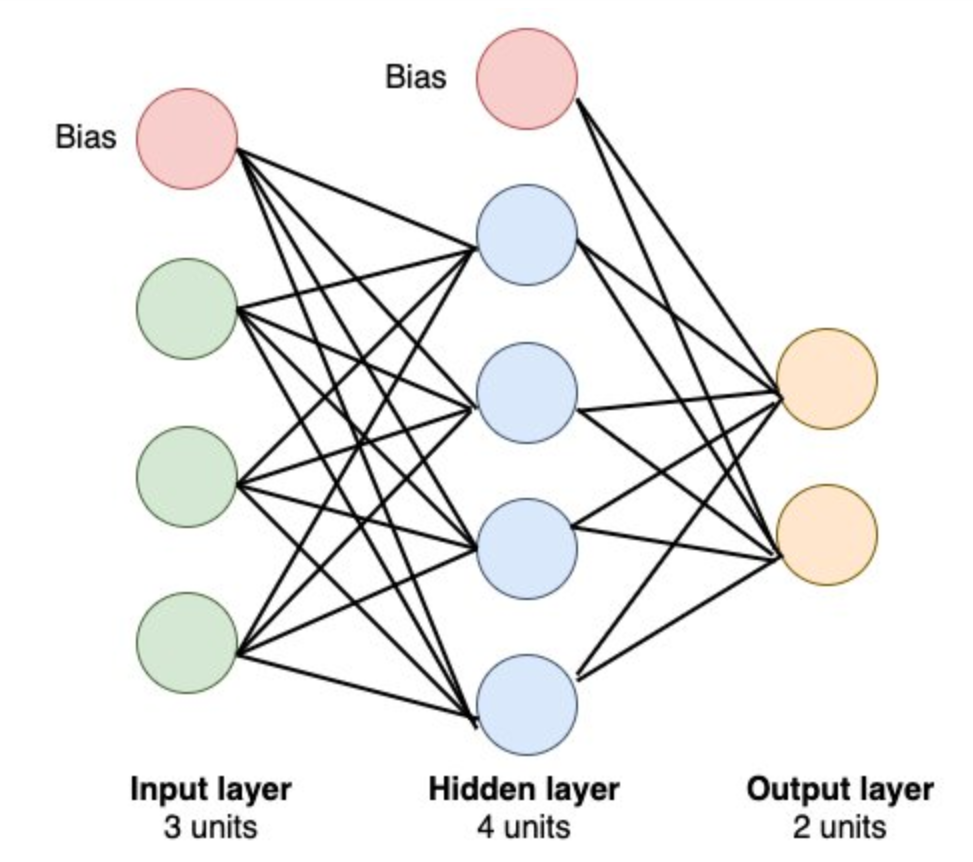
\includegraphics[width=300px]{MLP.png}
    \caption{An MLP with one hidden layer.}
    \label{fig:mlp}
\end{figure}

\subsection{What is an MPL?}

An MPL - multi layer perceptron - is a type of feed-forward artificial neural network (ANN) consisting of more multiple layers of perceptrons.\\
A perceptron is a single artificial neuron. It has a finite number of inputs with associated weights and one output. The output for a single perceptron is defined by the sum of all weights combined with an \hyperref[sec:activation_functions]{activation function}. Single perceptrons can only model linear functions (however with regard to multiple variables (inputs)) as the output is calculated as a polynomial of degree 1 of all inputs. However, with multiple layers of perceptrons we can also model non-linear functions, which is shown on the example of XOR in \hyperref[sec:solving_non_linear_problems_with_nns]{section \ref*{sec:solving_non_linear_problems_with_nns}}.

Note: You can also refer to an MLP as an ANN which has the following properties:
\begin{enumerate}
    \item Amount of layers $> 1$.
    \item All layers are fully connected layers.
\end{enumerate}

\subsection{Number of parameters in MPLs}

A parameter in a multi layer perceptron is one of the weights that are changed during training visualized by the lines between neurons.\\

We declare the following variables:
\begin{itemize}
    \item $l_{i}$: amount of neurons in layer $i$.
\end{itemize}

If $l_{i}$ is the amount of neurons in layer $i$ starting with the input layer being layer $1$, then the number of parameters in an MLP without biases is:

$$
    \sum_{i=1}^{n-1}l_{i}\cdot{l_{i+1}}
$$

If the MLP has biases in every layer, the amount of biases is calculated as the sum of neurons in all layers except the input layer. This is because as \hyperref[fig:mlp]{figure \ref*{fig:mlp}} shows, biases are usually connected to every neuron of a layer and input layers have no biases:

$$
    \sum_{i=2}^{n}l_{i}
$$

Therefore when calculating the amount of parameters in an MPL with biases in every layer, of course add up both terms.

\section{Feature map calculation in convolutional NN}

Feature map is a term mostly used to describe the output of a convolutional layer. We calculate one element of this output by calculating the dot-product of the convolutional kernel and the respective input features while centering the kernel on the feature to map.

\begin{figure}[h]
    \centering
    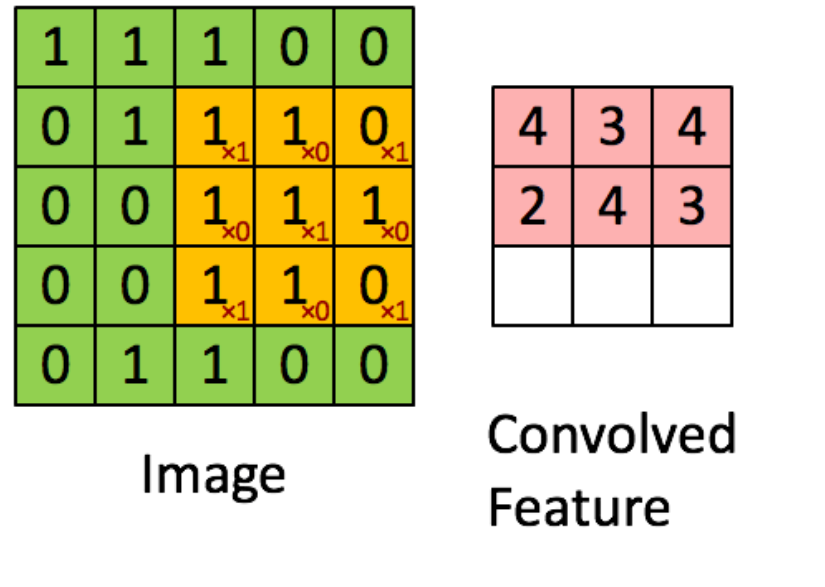
\includegraphics[width=250px]{feature_map_calulation.png}
    \caption{Calculation of a feature map with a $3 \times 3$ kernel with the values $(1, 0, 1, 0, 1, 0, 1, 0, 1)$}
    \label{fig:feature_map_conv_net}
\end{figure}

\section{Input and output sizes in ANNs}

The size of the input and the output layer in an ANN is predetermined by the problem to be solved. The input layer has as many neurons as the data has features. Of course we can use mechanisms for preprocessing our data first which would then change the dimensions of it's feature vectors and therefore also the number of neurons in the input layer. The size of the output layer is determined by the expected output. For a binary classification problem the output may be a single neuron. For classification with one-hot-encoding the number of neurons in the output layer is equal to the number of classes to predict.

\section{Activation Functions}
\label{sec:activation_functions}

An activation function is a function that is applied to the output of each node of a ANN. A simple activation function could be one that puts out either $0$ or $1$ depending on a threshold. Three more activation functions shall be presented in the following.

\subsection{ReLU}

The ReLU function can be used to only respect a neuron if it has a positive output. It's advantages are that it is easy to compute and favors the reduction of connections between nodes, which would be the case if a neuron is outputting a value less than $0$.

$$
    relu(x) =
    \begin{cases}
        \begin{rcases*}
            x & \quad x $>$ 0, \\
            0 & \quad x $\leq$ 0 \\
        \end{rcases*}
    \end{cases}
$$

\begin{figure}[h]
    \centering
    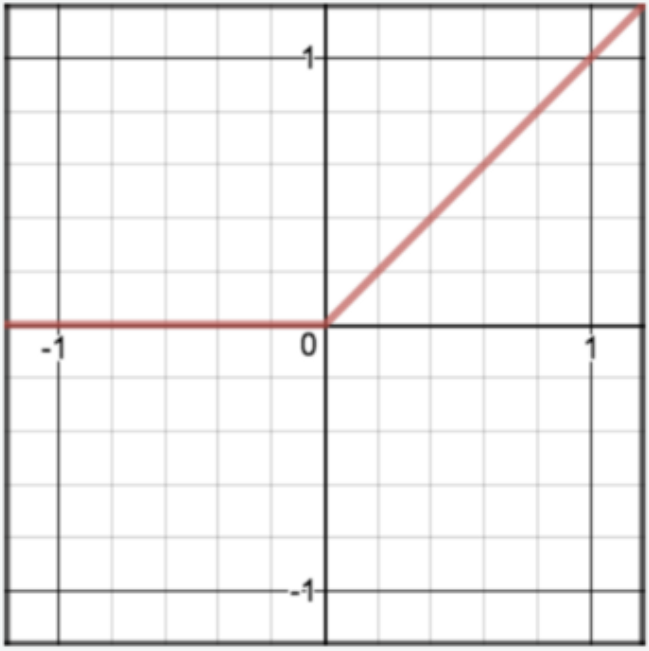
\includegraphics[width=150px]{ReLU.png}
    \caption{ReLU activation function}
    \label{fig:relu}
\end{figure}

\subsection{Sigmoid}

The sigmoid function produces values in the range from $0$ to $1$. Also the values are symmetric with respect to the y-axis. This is very helpful when the output of a node is supposed to be interpreted as a probability.

$$
    sigmoid(x) = \frac{1}{1 + e^{-x}}
$$

\begin{figure}[h]
    \centering
    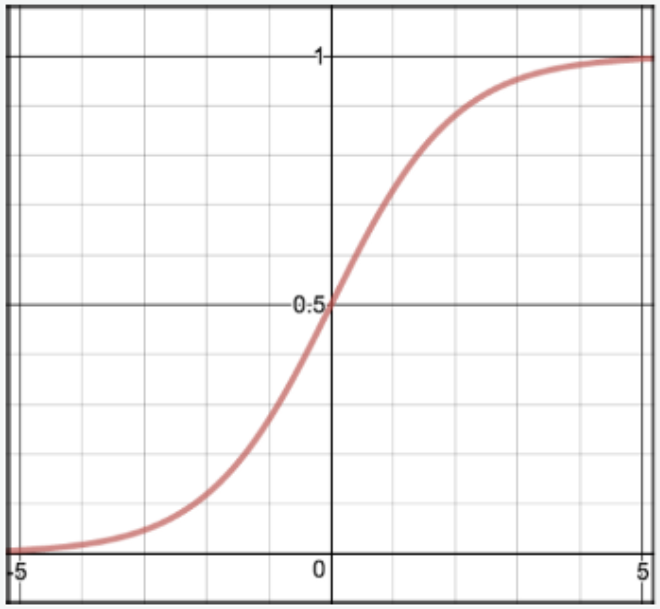
\includegraphics[width=150px]{sigmoid.png}
    \caption{Sigmoid activation function}
    \label{fig:sigmoid}
\end{figure}

\subsection{Softmax}

$$
    softmax(x)_{j} = \frac{e^{x}}{\sum_{k=1}^{K}e_{k}^{x}}
$$


The softmax function is a function that is typically applied to all output values of a NN for a classification problem. We assume that we have $K$ classes (output neurons) and an input $x$. The softmax function transforms the output values of each $k$-th neuron in a way that they all together add up to one and can therefore seen as probabilities for the corresponding class.

\begin{figure}[h]
    \centering
    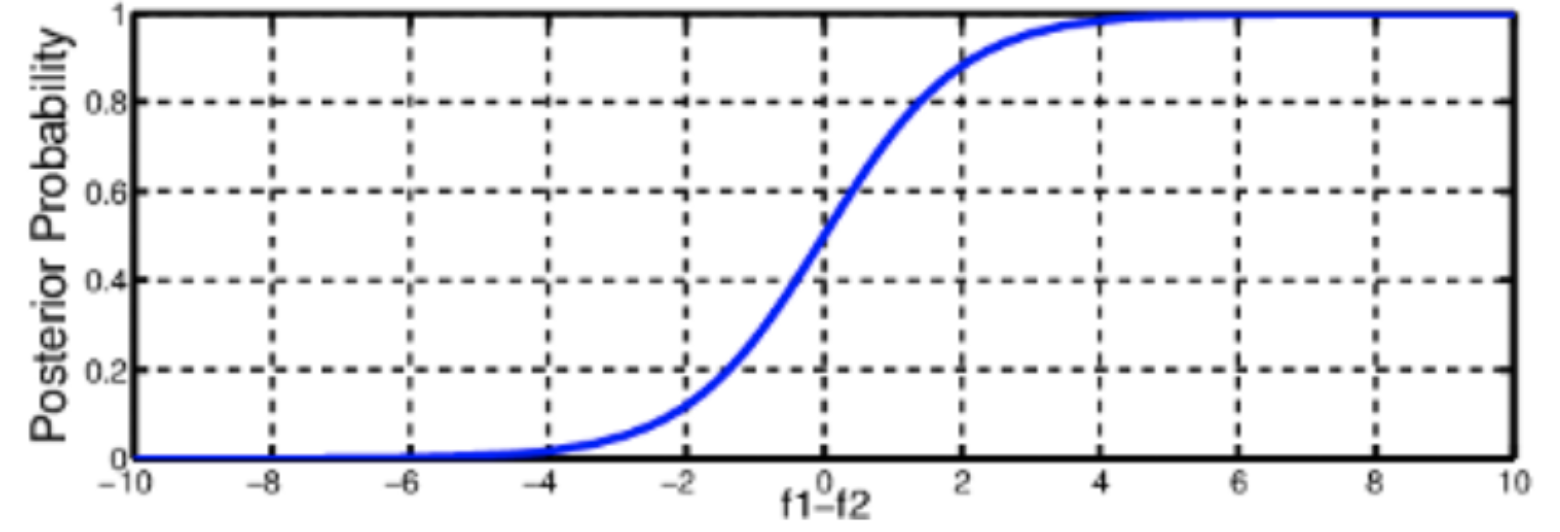
\includegraphics[width=300px]{softmax.png}
    \caption{Softmax activation function}
    \label{fig:softmax}
\end{figure}

\section{Solving non-linear problems with NNs}

\label{sec:solving_non_linear_problems_with_nns}

\begin{figure}[h]
    \centering
    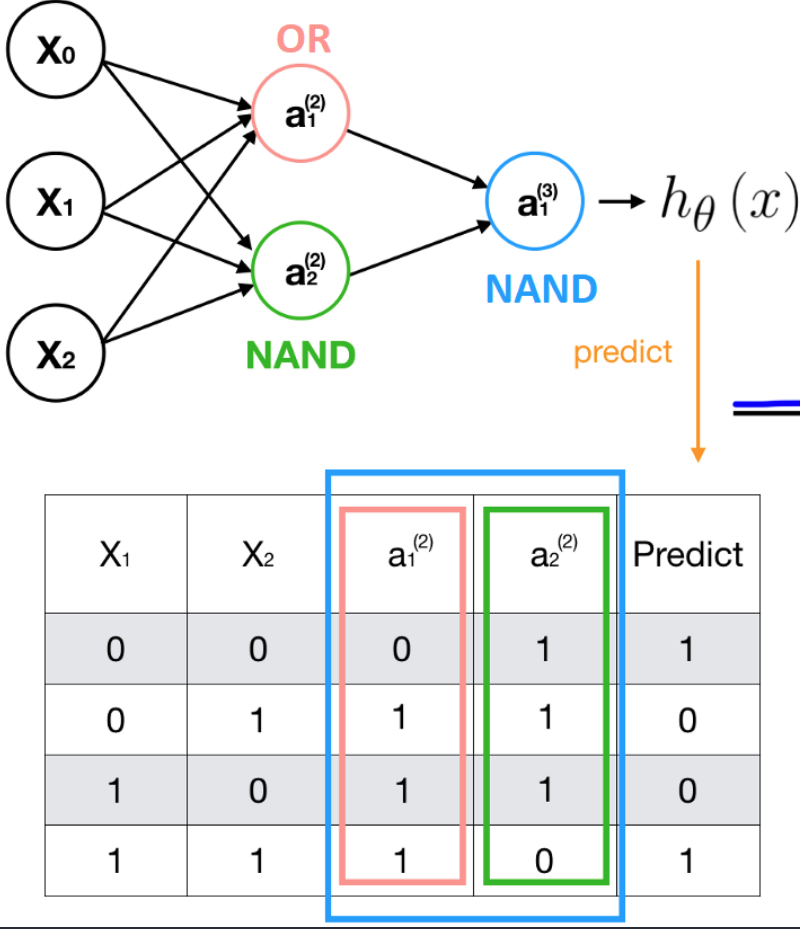
\includegraphics[width=300px]{mlp_xor.png}
    \caption{MLP for calculating XOR}
    \label{fig:mlp_xor}
\end{figure}

With a single \hyperref[sec:mlp]{perceptron} we can only fit linear functions. This is because a perceptrons output value is calculated as a linear function $output = a_{1} x_{1} + a_{2} x_{2} + ... a_{n} x_{n}$ of all it's $n$ inputs $x_{i}$ and weights $a_{i}$. However with multiple layers of perceptrons we can also fit non-linear functions. That means we can use multiple linear components (neurons) to build a non-linear model without explicitly using a polynomial model with degree $\geq 2$.

An example of this is the non-linear logical function XOR shown in figure \ref{fig:mlp_xor}. As XOR is a logical function the amount of its inputs is predetermined to be $2$ ($x_{1}, x_{2}$). We cannot model XOR with a single perceptron using $2$ inputs to that one perceptron. However we can model XOR as a combination of 3 neurons. These 3 neorons then themselves model OR, NAND and NAND which results in XOR as combination. The bias neuron $x_{0}$ shown in figure \ref{fig:mlp_xor} is unnecessary.

\section{K-means}

The $k$-means algorithm is an algorithm which takes a set of data points and a positive integer $k$ as input. It then clusters similar data points into $k$ clusters. It favors clusters with low variance and similar size. $k$ must be chose in the application context and might be the number of known classes of data points.\\

The algorithm works as follows:
\begin{enumerate}
    \item Randomly initialize $k$ points as \quotes{centers}" within the space of our data.
    \item Associate each data point with its closest \quotes{center}
    \item Update the centers to the center of all points associated with it.
    \item Repeat the re-centering for a fixed amount of iterations or until convergence.
\end{enumerate}

\section{Gradient Descent}

TODO: do this

\section{Hyperparameters of ML models}

\subsection{Batch Size}

Batch size is the number of data points shown to the net before the weights are adjusted using back-propagation. In real gradient descent the batch size is the dataset size. Then all weights are updated with regard to the mean error produced by all data points i.e. all data points affect each update of the weights directly. To increase learning speed we can also use batches of random sets of samples which will make us update more often with similar results.

\subsection{Epochs}

Epochs are the amount of times the net is shown the entire dataset while training.

\subsection{Learning Rate}

During back-propagation the parameters of the network are adjusted contrasting to the calculated error. The learning rate is a scalar that the error is multiplied with which therefore specifies to what extend the network shall learn. Too large learning rates can result in overshooting the minimum and non-convergence. Too Small learning rates can result in a slow learning process. In practice the learning rate is often chosen to be a value between 0.1 and 1. It is also possible to adjust the learning rate over time (often called decay) in order to learn faster in the beginning and then slow down the learning to smoothly approach the minimum of the loss function.

\subsection{Regularization}

Regularization is explained in \hyperref[sec:regularization]{section \ref*{sec:regularization}} in detail.

\subsection{Convolution Kernel Size}

When using convolutional layers in ANNs we use an $n \times n$ kernel (filter matrix). Usually an odd number is chosen for $n$ such that the kernel has a center, most popular is 3, sometimes 5. Then we slide the filter over the image such that each pixel has been in the center of the kernel once. We calculate the value of an output pixel, which is the pixel currently in the center of the kernel, as the dot-product of the kernel and the pixels of the image. Note that we would do this in multiple dimensions if we had a multi-channel image like RGB. Using convolutional layers can extract information like edges from the picture if the values for the elements of the kernel are chosen in a way that they calculate the gradient of adjacent pixels.

\subsection{Pooling Layers}

Pooling layers can be used in ANNs to down sample the feature maps i.e. reduce the amount of features. In general it is always better if data can be reduced while information is retained, as this decreases the number of nodes and therefore parameters in following layers and therefore speeds up the computation. Pooling layers typically use a $2 \times 2$ kernel with a stride of $2$. They therefore reduce the amount of features of an image by factor $4$. Pooling layers are often used after convolutional layers to decrease the size of the representation of the extracted features. In practice two types of pooling layers are most prominent:

\begin{itemize}
    \item \textbf{Max pooling layers} calculate the maximum value within the scope of the kernel.
    \item \textbf{Average polling layers} calculate the averyge value within the scope of the kernel.
\end{itemize}

\section{Logistic Regression and Cross Entropy}

TODO: do this


\section{Linear Regression and Normal Equation}

TODO: do this


\section{Decision Trees}

A decision tree is a binary tree that maps data points recursively to leaf nodes. Each leaf node is associated with one class and this way the result of traversing a decision tree with a given data point can be used for classification problems.\\
The interesting problem is how should a decision tree choose it's conditions in it's non-leaf nodes? As the tree is most efficient if the most information is extracted in each node, we recursively try to achieve that. We start with one root node and search e.g. with a grid search for a condition that maximizes the information gain at that node. Then we repeat for both child nodes. We stop at a node if it only contains data points of the same class or if we hit a given threshold of entropy or nodes.\\

Now lets look at how information gain is defined. To look at that we must first understand entropy. Entropy is value between 0 that shows the the uncertainty of a decision or put differently the mean information contained in one data point. If $p_{i}$ is the probability that a data point is an instance of class $i$ the entropy is calculated as follows:

$$
    H = -\sum_{i=1}^{N}p_i \log_2{(p_i)}
$$

It follows that the entropy is maximized i.e. equal to $1$ if the amount of data points belonging to one specific class is equal for all classes. Likewise the entropy is minimal i.e. equal to $0$ if all data points belong to the same class.\\

Information Gain is now defined as the loss of entropy per data point. The formula is as follows, where $w_{i}$ is the percentage of the data of the parent being mapped to child $i$ and $n$ being the the number of child nodes (in decision trees $n$ is always 2).

$$
    IG(Parent) =  H(Parent) - \sum_{i=1}^{n} w_{i} \cdot H(Child)
$$

In practice to avoid overfitting we would usually stop early i.e. we would not construct the entire tree until each leaf node has the entropy 0. Instead we would define limiting conditions like \textit{maximum tree depth}, \textit{maximum features} and \textit{minimum samples per leaf}.

\begin{figure}[h]
    \centering
    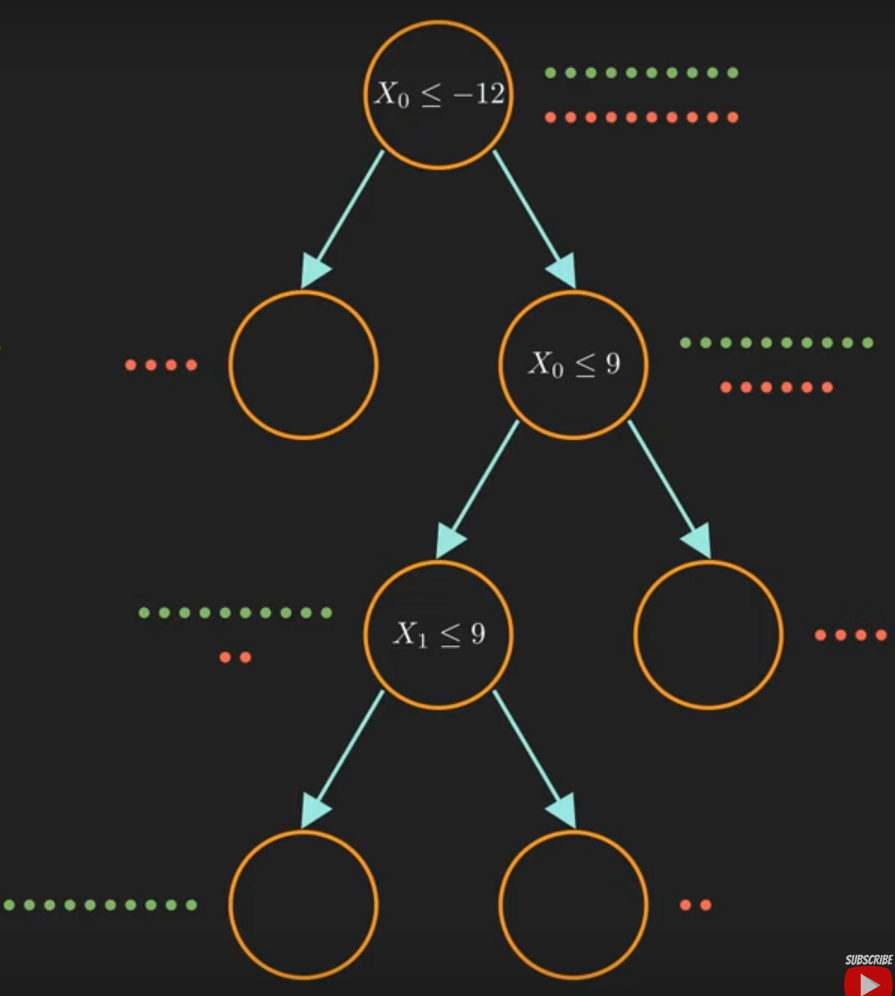
\includegraphics[width=300px]{decision_tree_classifier_1.png}
    \caption{Illustration of a simple decision tree for data with two features $x_{0}$ and $x_{1}$}
    \label{fig:mlp}
\end{figure}


\section{Random Forest}

Decision trees are highly sensible to the training data as their shape may be completely different for different training data. Therefore overfitting is a big issue. Random forest can solve this issue by using multiple decision trees on random subsets of the data and combining the prediction results. The algorithms for sampling and combining the trees here are \textit{bootstrapping} and \textit{aggregating}, which are also called \textit{bagging} in this combination.\\
Bootstrapping is performed by taking a random sample out of the dataset $n$ times. Here it it possible that a data point is chosen multiple times or never. This sampling is repeated $k$ times for the generation of a random forest with $k$ trees. Then a decision tree is build individually for each bootstrapped dataset.\\
When predicting on new unseen data the predictions of all trees are combined. For regression problems we calculate the mean, for classification problems the majority wins.

\section{K-nearest-neighbors}

K-nearest-neighbors (KNN) is also referred to as:

\begin{itemize}
    \item Instance-Based Learning,
    \item Lazy Learning,
    \item Non-Parametric Learning.
\end{itemize}

The main idea of KNN is to store the entire training dataset in a data structure and then when predicting a new value find the K most similar data points in the training data set. Then the target values of those K neighbors are aggregated. It follows that no training is needed. Now for the implementation of KNN the following has to be considered:

\begin{enumerate}
    \item How to store the training dataset for an efficient lookup? Of course we do not want to have to a linear search for finding the K neighbors.
    \item How to calculate the similarity of data points?
    \item How to aggregate the target values of the neighbors to one scalar prediction value?
\end{enumerate}

\subsection*{Dataset storage}

For an efficient lookup usually a kind of tree structure is used.

\subsection*{Calculation of similarity}

The most popular distance measures are:
\begin{itemize}
    \item Euclidean distance: The root of the sum of squared differences of the components of the feature vectors. Performs well on features of similar type e.g. height, width, weight.
    \item Manhattan distance: Sum of the absolute differences of the components of the feature vectors. Performs well on heterogenous features like age, sex, hair color.
\end{itemize}

\subsection*{Aggregation of Target Values}
Once the K nearest neighbors of a new data point have been found, their target variables have to be aggregated. For regression problems it is typical to take the mean or median. For classification problems it is typical to take the class which the majority of the neighbors have.


\end{document}
